\documentclass[journal]{IEEEtran}

\usepackage[pdfpagemode={UseOutlines},bookmarks=true,bookmarksopen=true,
   bookmarksopenlevel=0,bookmarksnumbered=true,hypertexnames=false,
   colorlinks,linkcolor={blue},citecolor={blue},urlcolor={blue},
   pdfstartview={FitV},unicode,breaklinks=true]{hyperref}

% *** MATH PACKAGES ***
\usepackage{amsmath,amssymb,bm}

% *** GRAPHICS RELATED PACKAGES ***
\ifCLASSINFOpdf
	\usepackage[pdftex]{graphicx}
	\graphicspath{{images/}}
	% \DeclareGraphicsExtensions{.pdf,.jpeg,.png}
\else
	\usepackage[dvips]{graphicx}
	\graphicspath{{images/}}
	% \DeclareGraphicsExtensions{.eps}
\fi

% *** SUBFIGURE PACKAGES ***
\ifCLASSOPTIONcompsoc
  \usepackage[caption=false,font=normalsize,labelfont=sf,textfont=sf]{subfig}
\else
  \usepackage[caption=false,font=footnotesize]{subfig}
\fi

\usepackage[pdftex,dvipsnames]{xcolor}
\usepackage{listings,xargs}
\usepackage[colorinlistoftodos,prependcaption,textsize=tiny]{todonotes}

\definecolor{dkgreen}{rgb}{0,0.6,0}
\definecolor{gray}{rgb}{0.5,0.5,0.5}
\definecolor{mauve}{rgb}{0.58,0,0.82}
\newcommand{\fsize}{\small}
%\newcommand{\fsize}{\tiny}
\newcommand{\tabsize}{4}

\lstset{frame=tb,
  language=C++,
%  aboveskip=0mm,
  belowskip=0mm,
  showstringspaces=false,
  columns=flexible,
  basicstyle={\fsize\ttfamily},
  numberstyle=\fsize\color{gray},
%  numbers=left,
  keywordstyle=\color{blue},
  commentstyle=\color{dkgreen},
  stringstyle=\color{mauve},
  breaklines=true,
  breakatwhitespace=true,
  tabsize=\tabsize
}

% correct bad hyphenation here
\hyphenation{op-tical net-works semi-conduc-tor}

\newcommand{\fref}[1]{\figurename~\ref{#1}}
\newcommand{\eref}[1]{(\ref{#1})}
\newcommand{\tref}[1]{\tablename~\ref{#1}}
\newcommand{\lref}[1]{LISTING~\ref{#1}}

\newcommandx{\improv}[2][1=]{\todo[linecolor=Plum,backgroundcolor=Plum!25,bordercolor=Plum,#1]{#2}}
\newcommand{\improvi}[1]{\improv[inline]{#1}}

\begin{document}

% paper title
\title{Acceleration of An SVM Classifier}

% author names and IEEE memberships
\author{Group 6: Yubo~Zhi (yz4116), Jiayang~Sun (js11815)}

% The paper headers
\markboth{ADSD Design Coursework}%
{ADSD Design Coursework}

% make the title area
\maketitle

\begin{abstract}
This course work aims to design and optimise a hardware Support Vector Machine (SVM) classifier on an embedded system using High Level Synthesis (HLS) language. The hardware implementation was optimised by various directives in HLS. In addition, the performance of software and hardware implementations were also assessed and compared in this excise.
\end{abstract}

\section{Introduction}

Dedicated hardware accelerators can perform a particular task faster then generalised software design. However, there are a few trade-offs associated with using hardware accelerators. In this exercise, an SVM classifier IP core was developed and optimised on a Xilinx ZYNQ SoC FPGA using Vivado HLS toolkit. The procedure of the design and optimisation will be explained in details. Finally, the performance differences between hardware and software implementations were evaluated and discussed.

\hfill \today

\section{IP core implementation}

\subsection{Overview}

\fref{fig:ip} shows the purposed SVM classifier accelerator architecture, designed according to \eref{eq:cls}.

\begin{align}
	f(\bm{x}) &= sgn \left( bias + \sum_{i=1}^{N_{SV}} \alpha_i k(\bm{{sv}_i}, \bm{x}) \right)
	\label{eq:cls}\\
	\text{where}~k(\bm{x}, \bm{y}) &= 2 tanh(\bm{x} \cdot \bm{y})
\end{align}

\begin{figure}[ht]
	\centering
	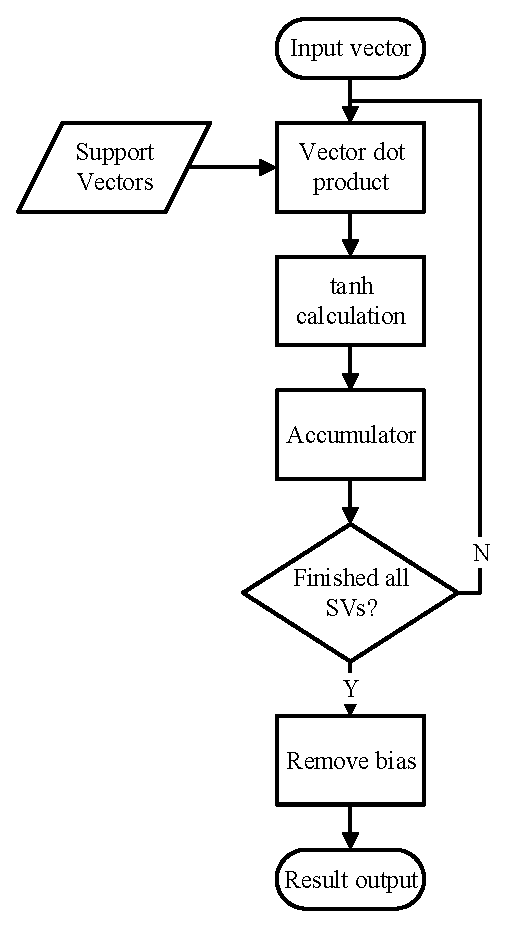
\includegraphics[width=0.6\columnwidth]{IP}
	\caption{Flow chart of purposed SVM classifier IP core}
	\label{fig:ip}
\end{figure}

According to the provided sample data, vectors have a width of 16 elements and there are 1050 support vectors. These numbers were replaced by macro definitions in the design, which can be easily adjusted to meet the properties of potentially other sample data.

\subsection{Dot product calculation}

Dot product between 2 vectors was calculated using the module designed previously in Part I.

\improvi{More descripsions}

\subsection{\texttt{tanh} calculation}

COordinate Rotation DIgital Computer (CORDIC) \cite{volder1959cordic} was used to calculate the \texttt{tanh} function.

\subsubsection{CORDIC}

CORDIC calculates trigonometric functions through vector rotation in 2-dimension space. It can be generalised to calculate \texttt{sinh} and \texttt{cosh} functions. The computations involved with CORDIC are simple integer addition, subtraction and shifting. This makes it suitable to use on a resource constrained embedded platform.

\subsubsection{Range and precision}

The precision of CORDIC can be improved by allowing more iterations, however, the input range of CORDIC is non-ideal. The CORDIC implementation used in this design has an input range of about $\pm 1.10$ radians, but the sample dataset can give an input as large as $83.6$ radians.

\improvi{The \texttt{fp\_tanh} conversion trick...}

\subsection{SVM classifier}

The top-level SVM classifier was designed according to the flow chart \fref{fig:ip}. It iterates through all Support Vectors, accumulates each result, finally output a boolean value according to the sign of accumulator after bias removal.

\improvi{Insert code here?}

\subsection{Hardware verification}

\subsubsection{Test bench}

The design of SVM classifier was verified using C simulation test benches.

\subsubsection{Reference generation}

\subsection{Design evaluation}

\improvi{the co-simulation is too long, only check with csim,show the result of synthesis}

\section{Performance optimisation}

\subsection{Interface optimisation}

\improvi{Array reshape, partition}

\subsection{Throughput optimisation}

\improvi{Pipeline, loop unrolling}

\subsection{Clock timing issue}

\improvi{Not meeting target clock rate.

Split long arithmetic operations on critical path.

use one array as a cache and add the array together to get the final answer.}

\subsection{Design verification}

\improvi{check the answer with golden file(Co simulation)?

talk about the initialisation of the array?
warning : the variable without initialisation?
arrar[n] = {0} ?}

\subsection{Design evaluation}

\improvi{Throughput, latency vs. Resource usage}

\section{System implementation}

\improvi{IP core packaging

Software testing with SDK}

\section{System evaluation}

\subsection{Performance and resource usage}

\subsection{Reflection and Limitation}

\iffalse

\begin{lstlisting}[caption={High level synthesis design for dot product},captionpos=b,label=lst:dotp]
#include <stdint.h>
#include "dotproduct.h"

void dotProduct(data_t x[N], data_t y[N],
                data_t *output)
{
        data_t acc = 0;
        uint32_t i;
loop:   for (i = 0; i != N; i++)
                acc += x[i] * y[i];
        *output = acc;
}
\end{lstlisting}



\begin{table}[!ht]
	% increase table row spacing, adjust to taste
	\renewcommand{\arraystretch}{1.3}
	\caption{Comparison between loop optimisation directives}
	\label{tbl:dir}
	\centering
	% Some packages, such as MDW tools, offer better commands for making tables
	% than the plain LaTeX2e tabular which is used here.
	\begin{tabular}{llll}
		\hline
			& None	& Pipeline	& Unroll \\
		\hline
		Latency	& 71	& 17	& 7	\\
		Interval	& 72	& 18	& 8	\\
		Co-simulation (average)	& 203	& 151	& 138	\\
		\hline
		BRAM\_18K	& 0	& 0	& 0	\\
		DSP48E	& 4	& 4	& 40	\\
		FF	& 1478	& 1477	& 990	\\
		LUT	& 7340	& 7339	& 1580	\\
		\hline
	\end{tabular}
\end{table}



\begin{figure*}[!t]
	\centering
	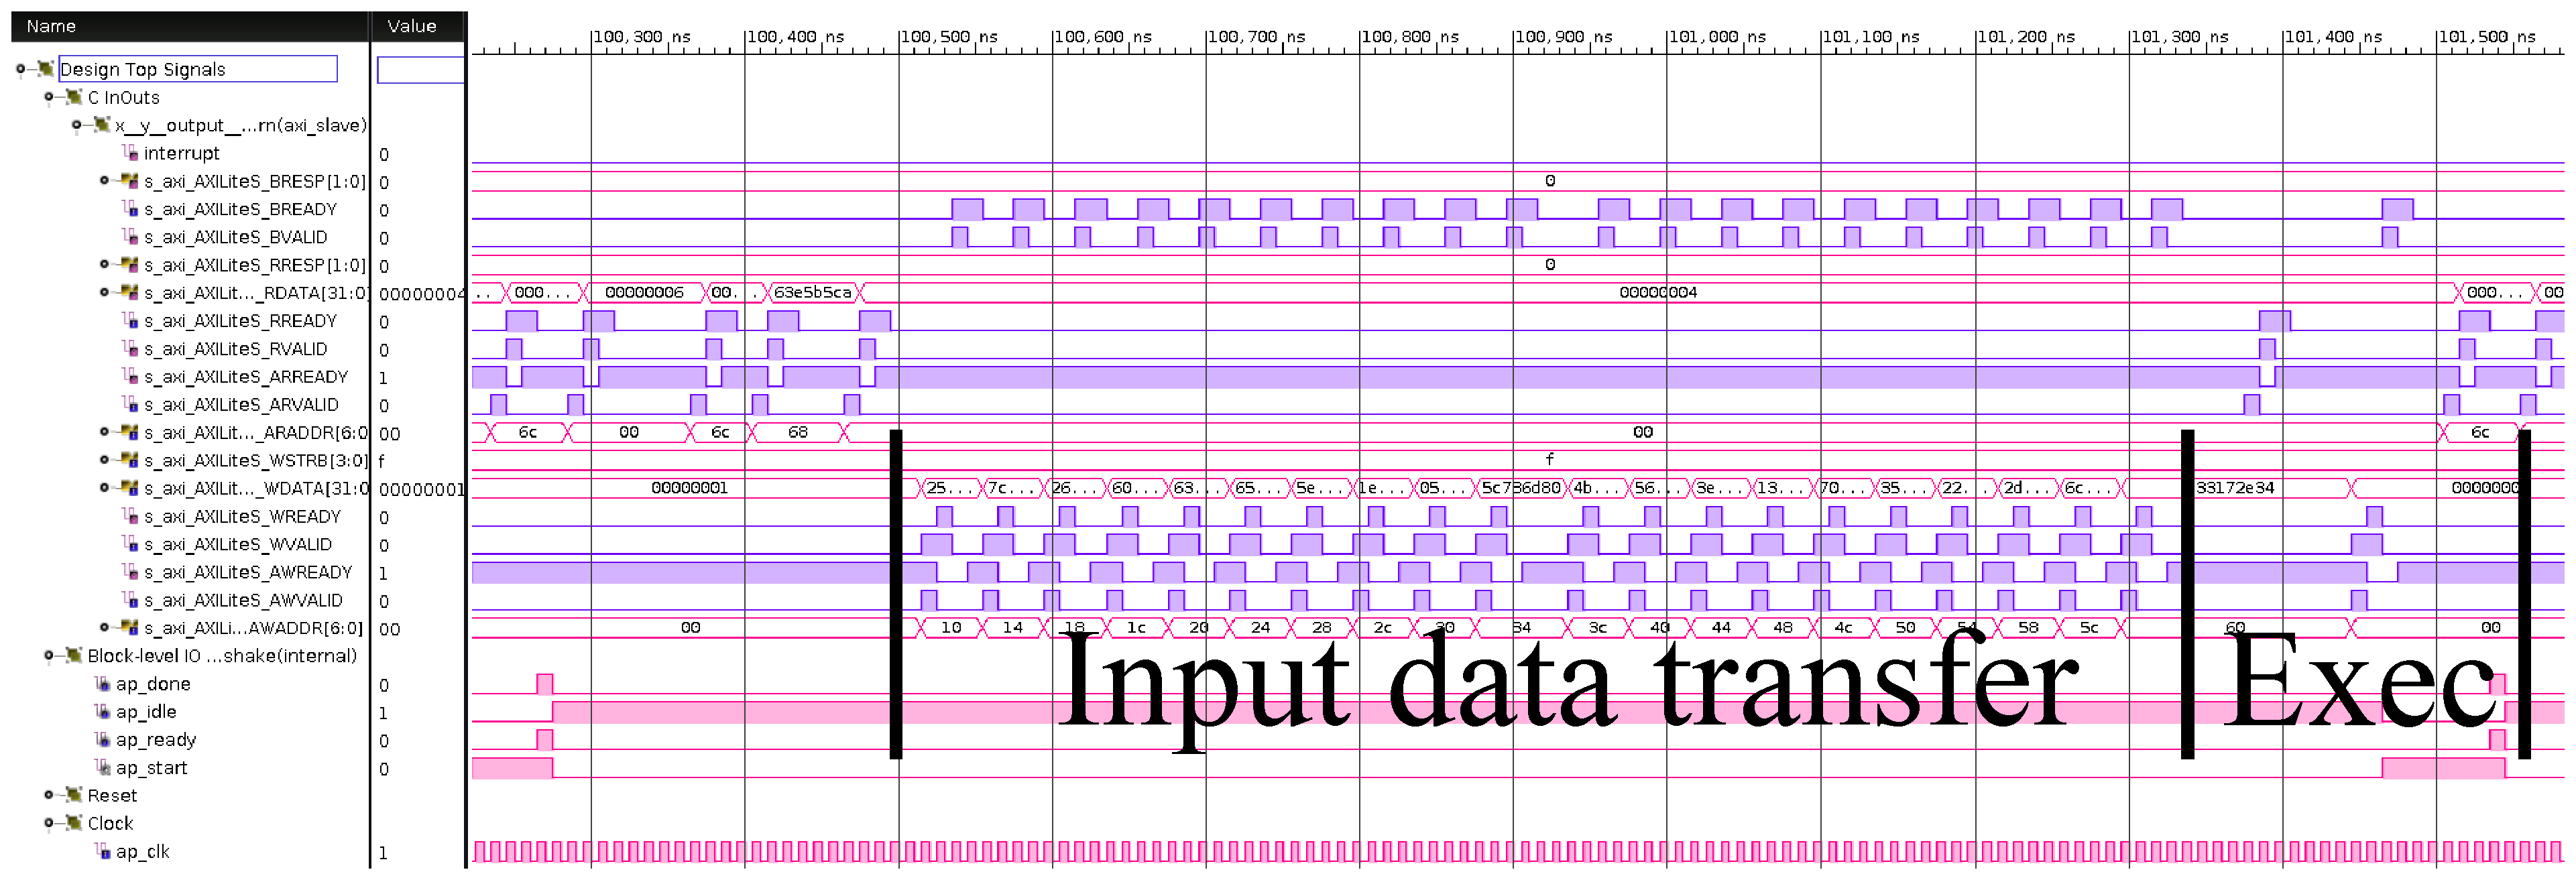
\includegraphics[width=\textwidth]{sim}
	\caption{Simulation waveform. Exec: actual execution time}
	\label{fig:sim}
\end{figure*}



\begin{table}[!ht]
	% increase table row spacing, adjust to taste
	\renewcommand{\arraystretch}{1.3}
	\caption{Resource utilisation of different data width}
	\label{tbl:reswidth}
	\centering
	% Some packages, such as MDW tools, offer better commands for making tables
	% than the plain LaTeX2e tabular which is used here.
	\begin{tabular}{ccccc}
		\hline
		Data width	& BRAM\_18K	& DSP48E	& FF	& LUT	\\
		\hline
		8	& 0	& 10	& 377	& 393	\\
		16	& 0	& 10	& 697	& 745	\\
		32	& 0	& 40	& 990	& 1580	\\
		64	& 0	& 160	& 2250	& 3130	\\
		\hline
	\end{tabular}
\end{table}

\fi

\section{Conclusion}

By evaluating the performance data of software and hardware implementation of the same algorithm, the advantages, use case and limiting factors of using hardware accelerators were investigated. Although the computation speed of dedicated hardware accelerator can be faster than software implementation, the data transfer performance may limit the actual efficiency.

The data transfer inefficiency may be improved by using another type of interface, e.g. the AXI4-Stream interface. It transfers data in a sequential streaming manner, would be better than 10 discrete register data transfers.

% References section
\bibliographystyle{IEEEtran}
\bibliography{Reference}

% that's all folks
\end{document}
